\chapter{Sistema Embarcado}
\label{cap:sistema-embarcado}

\section{Casos de Uso}
Descrição de cada caso de uso e como o usuário irá interagir com o sistema

\section{Microcontrolador}
A escolha da unidade de processamento central é um dos pilares para o desenvolvimento deste componente, visto que o microcontrolador deve balancear restrições físicas e elétricas com a demanda por processamento de dados em tempo real. Desta forma, realizou-se uma comparação entre duas principais arquiteturas concorrentes no cenário de sistemas distribuídos embarcados: o microcontrolador Espressif ESP32 e o STMicroelectronics STM32F405RG.

O dimensionamento da topologia de alimentação elétrica do sistema é diretamente impactado pelas características de consumo do circuito integrado. A arquitetura Xtensa do ESP32 demonstra um consumo energético mais elevado. Mesmo quando os módulos de radiofrequência nativos (Wi-Fi e Bluetooth) são completamente desativados via \textit{software}, o núcleo consome continuamente entre 30 mA e 50 mA apenas para a manutenção do agendador do sistema operacional de tempo real (FreeRTOS) em estado de ociosidade \cite{esp32_datasheet}. 

Quando associado aos picos transientes de corrente demandados pela transmissão de longo alcance via rádio, este comportamento impõe a necessidade de uma arquitetura de regulação de tensão mais complexa com conversores chaveados e capacitores baixa resistência em série equivalente (ESR) para mitigar quedas abruptas de tensão e instabilidades térmicas na placa.

Em contrapartida, a arquitetura ARM Cortex-M4 presente no STM32F405RG foi projetada sob o paradigma de eficiência para baixo consumo. Operando em sua frequência máxima de 168 MHz, o dispositivo apresenta um consumo dinâmico previsível situado na faixa de 30 mA a 40 mA, mantendo uma dissipação térmica estável e eliminando a exigência de malhas complexas de alívio térmico ou dissipadores na placa-base. \cite{STM32F405RG_datasheet}

O ESP32 apresenta elevada capacidade de processamento por meio de sua arquitetura \textit{Dual-Core} com dois núcleos operando a 240 MHz (Xtensa LX6). Esta característica possibilita o isolamento completo de tarefas através do escalonamento simétrico, alocando o processamento de baixo nível e a leitura de sensores em barramentos I2C/SPI ao Core 0, enquanto o gerenciamento da máquina de estados (FSM) e o orquestrador principal executam no Core 1. Essa separação impede que as latências de escrita de arquivos em cartões de memória provoquem perda de amostras de dados. No entanto, o seu coprocessador de ponto flutuante é menos otimizado e a arquitetura de cache do FreeRTOS introduz pequenas variações de latência (\textit{jitters}).

Por outro lado, o STM32F405RG adota um único núcleo operando a 168 MHz, porém integra uma Unidade de Ponto Flutuante (FPU) nativa implementada diretamente por \textit{hardware} \cite{STM32F405RG_datasheet}. Durante o cálculo de filtros matemáticos complexos, a FPU executa as operações de ponto flutuante de forma quase instantânea. Ademais, a arquitetura ARM fornece um determinismo de \textit{hardware} em tempo real superior, assegurando que interrupções críticas associadas aos sensores sejam atendidas com latências fixas e previsíveis.

A integração física e lógica com múltiplos periféricos síncronos e assíncronos requer controladores de barramento robustos e isolados de ruído. O ESP32 emprega uma matriz de comutação de GPIO altamente flexível, permitindo o mapeamento de pinos lógicos I2C, SPI e UART para praticamente qualquer terminal físico do encapsulamento, o que simplifica o desenvolvimento do \textit{layout} de trilhas da placa de circuito. Contudo, os controladores internos de barramento da família Espressif historicamente apresentam limitações e anomalias de comportamento em silício sob condições de alta carga de dados, exigindo rotinas complexas de tratamento de exceções no \textit{software} para evitar travamentos do barramento em caso de falhas de sincronismo de um sensor \cite{esp32_gpio_anomalies}.

Já o STM32F405RG conta com periféricos de comunicação dedicados com posições de pinos imutáveis. Seus controladores I2C, SPI e USART são blindados internamente em \textit{hardware}, apresentando maior imunidade a ruídos. Adicionalmente, o dispositivo dispõe de um barramento nativo de entrada e saída digital segura (SDIO) por \textit{hardware} \cite{STM32F405RG_datasheet}. A gravação e a persistência de registros de voo através de uma interface SDIO dedicada alcança taxas de transferência substancialmente superiores e com maior confiabilidade do que a emulação de cartões através do protocolo SPI genérico tipicamente implementada em plataformas baseadas no ESP32.

A análise indica que, para o cenário deste sistema, desprovido da necessidade de conectividade sem fio de curto alcance nativa, o ecossistema STM32 alinha-se melhor aos requisitos de determinismo, tolerância a falhas e confiabilidade exigidos.

Contudo, apesar das vantagens de \textit{hardware} apresentadas pela plataforma ARM, o microcontrolador ESP32 foi selecionado para a implementação final do protótipo deste trabalho devido à viabilidade de execução, destacando-se na ampla acessibilidade local aos componentes e módulos de desenvolvimento, no menor custo relativo de instrumentação e na robustez das cadeias de suprimentos disponíveis, garantindo o cumprimento dos prazos.

Com esta decisão, iniciou-se o processo de desenho do esquemático do circuito eletrônico, representado com o microcontrolador na Imagem \ref{fig:mc_scheme}. Vale citar que, para melhor manutenção, simplicidade e devido a motivos de acessibilidade, o sistema será implementado a nível de módulos comerciais. Ou seja, os componentes serão todos \textit{Through-hole technology} (THT) soldados a uma placa caseira com trilhas em cobre.

\begin{figure}[ht]
    \centering
    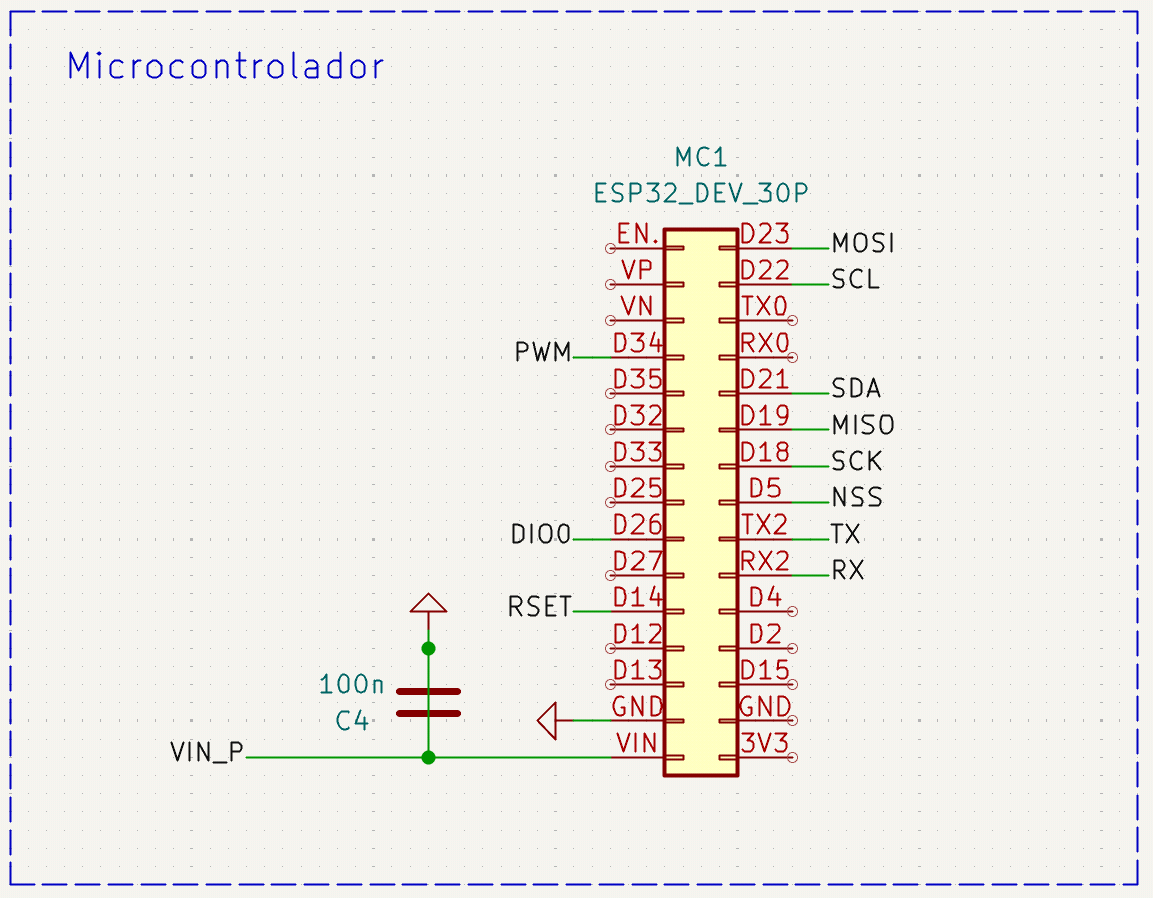
\includegraphics[width=0.9\textwidth]{images/mc_scheme.png}
    \caption{Esquemático Microcontrolador} \label{fig:mc_scheme}
\end{figure}

Por fim, para amenizar possíveis quedas de tensão em momentos de alta demanda da corrente, anexou-se um capacitor cerâmico de $100 nf$ em paralelo com a entrada VIN do ESP32. Por mais que módulos comerciais como o ESP32 Dev Kit já tenham sistemas integrados de controle energético, é importante garantir que não haja renícios forçados por subtensão (\textit{brownout}).

\section{Sensores e Módulos}
A seleção dos módulos de aquisição do sistema embarcado foi especificamente motivada pelos requisitos funcionais de telemetria. Conforme estabelecido previamente na Tabela \ref{tab:dados-requisitados}, o hardware em nível físico deve ser capaz de prover a aceleração no eixo da gravidade, a atitude espacial da aeronave, a velocidade relativa ao solo e a razão de subida da aeronave. Para satisfazer simultaneamente o escopo analítico das equipes de Cargas, Desempenho e Estabilidade, o sistema de aquisição deve consolidar componentes que operem sob margens de confiabilidade, lidando com os ruídos mecânicos e elétricos característicos do ambiente de voo.

Para o fornecimento dos dados de atitude tridimensional e do vetor de aceleração da gravidade, o projeto exige a implementação de um Sistema de Referência de Atitude e Proa (AHRS). Em ciclos de desenvolvimento passados, componentes de 6 graus de liberdade (6-DOF), a exemplo do legado MPU6050, figuraram como escolhas padrão \cite{tinyml_flight_phases}. Contudo, a ausência de um magnetômetro integrado neste encapsulamento impede a correção do vetor magnético terrestre, resultando na acumulação progressiva de erro matemático (\textit{drift}) no eixo de guinada. 

Outra alternativa amplamente adotada na instrumentação de baixo custo é o sensor BNO055, que integra 9 eixos e um coprocessador para fusão sensorial em hardware \cite{BNO055_datasheet}. Embora essa solução reduza drasticamente o esforço computacional do microcontrolador, sua arquitetura fechada impede a aplicação de filtros customizados e a escolha do componente onde a atitude será inferida, forçando o sistema a enviar pacotes maiores pela rede LoRa.

Desta forma, o presente sistema adota o módulo ICM-20948 como Unidade de Medição Inercial (IMU) primária. Trata-se de uma arquitetura de 9 eixos (acelerômetro, giroscópio e bússola) que entrega dados brutos de boa fidelidade. A associação física do magnetômetro ao silício, somada ao baixo perfil de ruído térmico e mecânico reportado pelo fabricante, confere ao barramento de comunicação uma amostragem satisfatoriamente limpa \cite{ICM-20948_datasheet}.

As análises conduzidas pelo subsistema de Desempenho e a validação do envelope de voo pelo subsistema de Cargas requerem a coleta de dados de translação aerodinâmica e referencial de pista. A aferição da velocidade relativa ao solo é atendida pela integração de um módulo receptor de Sistemas Globais de Navegação por Satélite (GNSS). Módulos legados, como o NEO-6M, limitam-se ao rastreamento primário da constelação GPS com taxas de atualização de apenas 1 Hz a 5 Hz \cite{NEO-6M_datasheet}, induzindo uma latência inaceitável para a dinâmica de manobras das aeronaves. Portanto, selecionou-se o receptor NEO-8M, que suporta o rastreio simultâneo de múltiplas constelações (GPS, GLONASS, Galileo) e fornece atualizações em frequências de até 10 Hz, assegurando a confiabilidade, a precisão posicional e o sincronismo temporal dos vetores de velocidade \cite{NEO-8M_datasheet}.

Por fim, a derivação da razão de subida e a correção da leitura altimétrica fornecida pelo GNSS demandam o monitoramento da pressão atmosférica estática. Soluções comerciais genéricas voltadas para a Internet das Coisas (IoT), como o BMP280, apresentam um piso de ruído e uma variação de medida que comprometem a precisão da aquisição \cite{BMP280_datasheet}. Portanto, adotou-se o módulo MS5611, que fornece uma resolução altimétrica efetiva na escala de centímetros \cite{MS5611_datasheet}. Essa informação é então utilizada para atenuar as margens de erro intrínsecas ao posicionamento por satélite no eixo vertical.

TODO: Tabelas comparativa

Os \textit{footprints} dos componentes comerciais foram desenhados conforme os \textit{datasheets} de cada módulo. Além disso, os sensores foram adicionados ao esquema de circuito do hardware, apresentado na Imagem \ref{fig:sensor_scheme}.

\begin{figure}[ht]
    \centering
    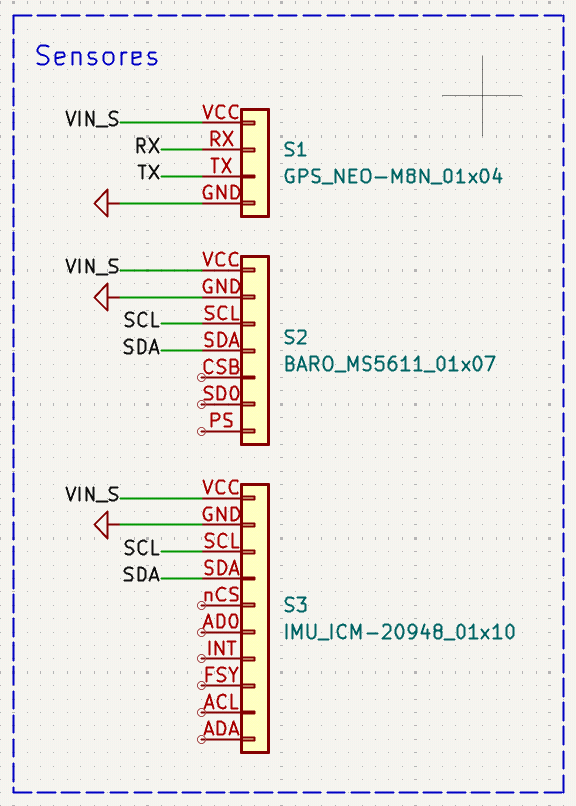
\includegraphics[width=0.55\textwidth]{images/sensors_scheme.png}
    \caption{Esquemático dos Sensores} \label{fig:sensor_scheme}
\end{figure}

Com os sensores determinados e os protocolos seriais identificados, seguiu-se para o próximo passo de determinar os componentes de comunicação. Estes, serão também módulos comerciais, porém com outro escopo de decisão e implementação.

\section{Componentes de Comunicação}
Para este sistema, existem três componentes de comunicação: o módulo de transmissão LoRa, a interface PWM com o receptor da aeronave e um \textit{buzzer} ativo para alertas sonoros.

Para a interface PWM, a necessidade é de apenas um barramento para o sinal modular e um barramento para compartilhamento do GND. Visando valorizar a integração da placa com o sistema de controle existente, utilizou-se de um trio de cabos AWG 24 com conctores fêmeas. Esse trio comumente abrange o sinal, o terra e o positivo.

Aqui, surge a oportunidade de ligar o sistema embarcado no mesmo sistema de alimentação do sistema de controle, aproveitando da bateria e componentes já existentes. Esta possibilidade será melhor discutida mais à frente no texto.

Para o módulo LoRa, a principal restrição se dá pelas normas de frequências permitidas para operação \cite{norma_frequencias}. Das opções comercialmente disponíveis, a única variação permitida para operação livre no Brasil é a de frequência $915 MHz$. 

Além disso, o acesso aos módulos pode ser relativamente custoso financeiramente. Portanto, a comparação entre os principais módulos que atendem ao requisito de frequência permitida se deu pelo valor e compatibilidade com o microcontrolador escolhido, como visto na Tabela \ref{tab:modulos_lora}.

Dessa forma, o módulo escolhido foi o SX1276, sendo a Figura \ref{fig:comm_scheme} a adição do LoRa, do PWM e do \textit{buzzer} ao esquemático do projeto.

\begin{figure}[ht]
    \centering
    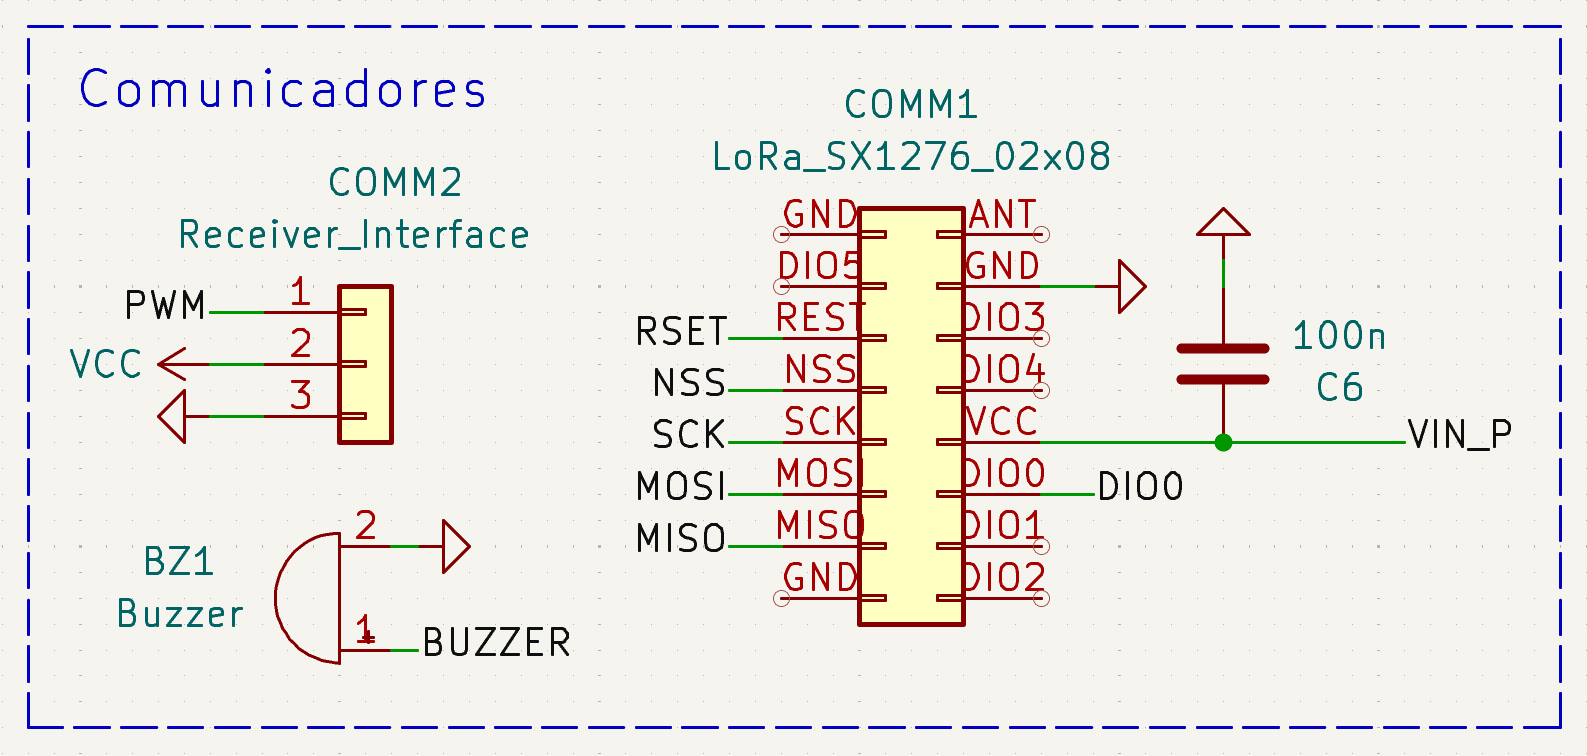
\includegraphics[width=0.9\textwidth]{images/comm_scheme.png}
    \caption{Esquemático dos Comunicadores} \label{fig:comm_scheme}
\end{figure}

Por fim, vale citar que o módulo LoRa SX1276 exige correntes de pico consideráveis --característica intrínseca dos transmissores de alto alcance --, aproximando-se de $120 mA$ quando configurado para transmitir na potência máxima de $+20 dBm$ \cite{SX1276_datasheet}. Por isso, adicionou-se um capacitor de $100 nf$ em paralelo à entrada VCC do módulo, criando um amortecimento aos picos de potência que o LoRa irá provocar. O pico de consumo do SX1276 não é um fator bloqueante, mas se torna um ponto de atenção para o dimensionamento da camada de alimentação energética do sistema.

\section{Rede de Distribuição de Potência e Dimensionamento Elétrico}
O projeto de hardware para um sistemas aviônicos embarcado planejamento criterioso da rede de distribuição de potência (PDN). Em VANTs, as oscilações elétricas induzidas por atuadores mecânicos do sistema de controle e as restrições de dissipação térmica representam desafios para a estabilidade do microcontrolador e componentes.

\subsection{Definição da Fonte e Levantamento de Carga}
O subsistema embarcado recebe energia diretamente dos pinos de barramento do receptor de rádio acoplado ao sistema de controle da aeronave. Esse barramento é alimentado por uma bateria de fosfato de ferro-lítio (LiFePO4) de duas células (2S), que apresenta uma tensão nominal de $6,6 V$, podendo atingir $7,2 V$ quando em estado de carga máxima \cite{LiFePO4}.

Para o dimensionamento físico da rede elétrica, realizou-se um levantamento da demanda de corrente do hardware em regime de operação. O microcontrolador base terá um consumo típico estabilizado, mas demandará correntes complementares durante as rotinas de inicialização \cite{esp32_datasheet}. Simultaneamente, o módulo LoRa operando na banda de $915 MHz$ exige uma demanda instantânea de corrente de aproximadamente $120 mA$ durante os ciclos de transmissão em potência máxima de $+20 dBm$ \cite{SX1276_datasheet}. Estima-se que, sob condições normais de operação, o pico de consumo total do arranjo de processamento, sensores e rádio situa-se em aproximadamente $700 mA$.

\subsection{Problemática Térmica e Ruído Conduzido}

A imposição de rebaixar o nível de tensão de até $7,2 V$ para o patamar operacional de $3,3 V$ sob uma corrente contínua de $0,7 A$ introduz a necessidade de atenção às restrições térmicas. Caso a arquitetura adotasse uma regulação estritamente linear por meio de componentes monolíticos padrão — como o regulador AMS1117-3.3 —, a potência dissipada exclusivamente sob a forma de calor ($P_D$) seria calculada pela Lei de Joule:

$$P_D = (V_{in} - V_{out}) \cdot I$$
$$P_D = (7,2\text{ V} - 3,3\text{ V}) \cdot 0,7\text{ A} = 2,73\text{ W}$$

Considerando que o encapsulamento físico desses reguladores lineares suporta um limite prático de dissipação térmica próximo a $1,0 W$ em ambientes fechados, a exigência de $2,73 W$ sobrecarregaria o componente em poucos segundos. Esse excesso de calor ativaria os circuitos internos de proteção térmica, resultando no desligamento completo do sistema de telemetria durante o voo \cite{thermal_management}.

Além da restrição térmica, o barramento elétrico é compartilhado com os servomotores da aeronave por meio do receptor. O acionamento dinâmico dessas cargas indutivas gera picos de força contraeletromotriz e quedas severas na tensão de entrada. Sem o devido isolamento elétrico, os disparos rápidos de transmissão do módulo LoRa provocam quedas localizadas de voltagem, colocando o microcontrolador em um estado de \textit{brownout} \cite{the_art_of_electronics}.

\subsection{Arquitetura de Distribuição de Energia \textit{Dual-Rail}}

Para contornar as limitações térmicas e isolar os ruídos conduzidos, implementou-se uma topologia de alimentação do tipo \textit{Dual-Rail}, distribuindo a energia em duas vias independentes:

\begin{itemize}
  \item{\textbf{Trilha de Potência:} Direcionada aos componentes de consumo elevado e perfil ruidoso, nominalmente o microcontrolador e o transceptor de rádio. Utiliza-se o mini-360, um conversor \textit{Step-Down} chaveado que reduz a tensão de entrada para $3,3 V$ com eficiência superior a $85\%$. Esse módulo suporta picos de corrente de até $2 A$ sem gerar dissipação térmica expressiva, garantindo a estabilidade operacional dos módulos de comunicação \cite{mini360_datasheet}.}
  \item{\textbf{Trilha Sensível:} Dedicada exclusivamente aos componentes de instrumentação (IMU, barômetro e GNSS), cujo consumo somado é baixo. Um regulador linear de baixa queda de tensão (LDO), alimentado diretamente pela fonte primária, fornece uma saída isolada em $3,3 V$. Devido à baixa corrente dos sensores, o calor gerado é mínimo. A vantagem desta abordagem reside na pureza espectral do sinal elétrico, visto que os LDOs barram os ruídos de alta frequência provenientes do chaveamento do conversor \textit{Buck} e das transmissões de rádio, preservando a integridade das leituras analógicas e digitais dos sensores \cite{power_delivery_network_design}.}
\end{itemize}

\subsection{Dimensionamento de Filtros e Análise de Transientes}

Para garantir o amortecimento dos transientes de carga e prevenir oscilações que violem os limites operacionais dos circuitos integrados, o dimensionamento dos capacitores de desacoplamento e armazenamento local baseou-se na equação fundamental da capacitância em função da variação temporal de corrente e tensão:

$$C = I \cdot \frac{\Delta t}{\Delta V}$$

No nó de transmissão de $3,3 V$ (compartilhado pelo processador e pelo rádio), estima-se que o degrau de corrente abrupto ($I$) atinja $0,62 A$ durante as janelas de calibração e envio de pacotes. Sabendo que o limite inferior de integridade dos circuitos de radiofrequência ocorre em $3,0 V$, a queda de tensão máxima tolerável ($\Delta V$) no barramento é de $3,3\text{ V} - 3,0\text{ V} = 0,3\text{ V}$. Assumindo um tempo de resposta aproximado ($\Delta t$) de $200\,\mu\text{s}$ para que a malha de realimentação do conversor \textit{Buck} compense a demanda repentina \cite{mini360_datasheet}, o cálculo da capacitância necessária resulta em:

$$C = 0,62\text{ A} \cdot \frac{0,0002\text{ s}}{0,3\text{ V}} \approx 413\,\mu\text{F}$$

Para suprir essa demanda com margem de segurança, adotou-se um capacitor eletrolítico de $470\,\mu\text{F}$ posicionado fisicamente próximo aos pinos de alimentação do circuito de controle. O componente selecionado apresenta uma resistência série equivalente de $150\text{ m}\Omega$ ($\text{ESR} = 0,15\,\Omega$) \cite{capacitor_esr}. Para mitigar a queda de tensão resultante dessa resistência e compensar a alta Indutância Série Equivalente (ESL) típica desse tipo de encapsulamento, adicionou-se um capacitor cerâmico de $100\text{ nF}$ em paralelo. Essa associação reduz a impedância total do conjunto em frequências elevadas, impedindo que flutuações de tensão indutivas ou resistivas reiniciem o processamento.

Na entrada primária de 6,6 V, o sistema deve suportar transientes mecânicos mais lentos gerados pelos servomotores, cujos distúrbios na linha de transmissão duram cerca de $1\text{ ms}$ ($\Delta t = 0,001\text{ s}$) \cite{servo_disturbio}. Considerando a corrente máxima de regime da placa de telemetria ($I = 0,7\text{ A}$) e estabelecendo uma margem de queda de tensão estritamente segura de $\Delta V = 1,0\text{ V}$ para manter a entrada dos reguladores acima do limite de \textit{dropout}, aplica-se a relação matemática:

$$C = 0,7\text{ A} \cdot \frac{0,001\text{ s}}{1,0\text{ V}} = 700\,\mu\text{F}$$

Visando trazer robustez ao hardware contra os altos consumos provenientes dos esforços nas superfícies de comando da aeronave, implementou-se um capacitor eletrolítico de $1000\,\mu\text{F}$ com isolação nominal de $16 V$ na entrada da placa. Em paralelo a esse componente, adicionou-se um capacitor cerâmico de $100\text{ nF}$ focado na supressão de ruídos de alta frequência induzidos pelos motores CC dos servos, completando a barreira de proteção eletromagnética do sistema embarcado \cite{electromagnetic_compatibility_engineering}.

Com a arquitetura idealizada, realizou-se a adição dos componentes ao esquemático da placa de circuito, conforme Imagem \ref{fig:power_scheme}

\begin{figure}[ht]
    \centering
    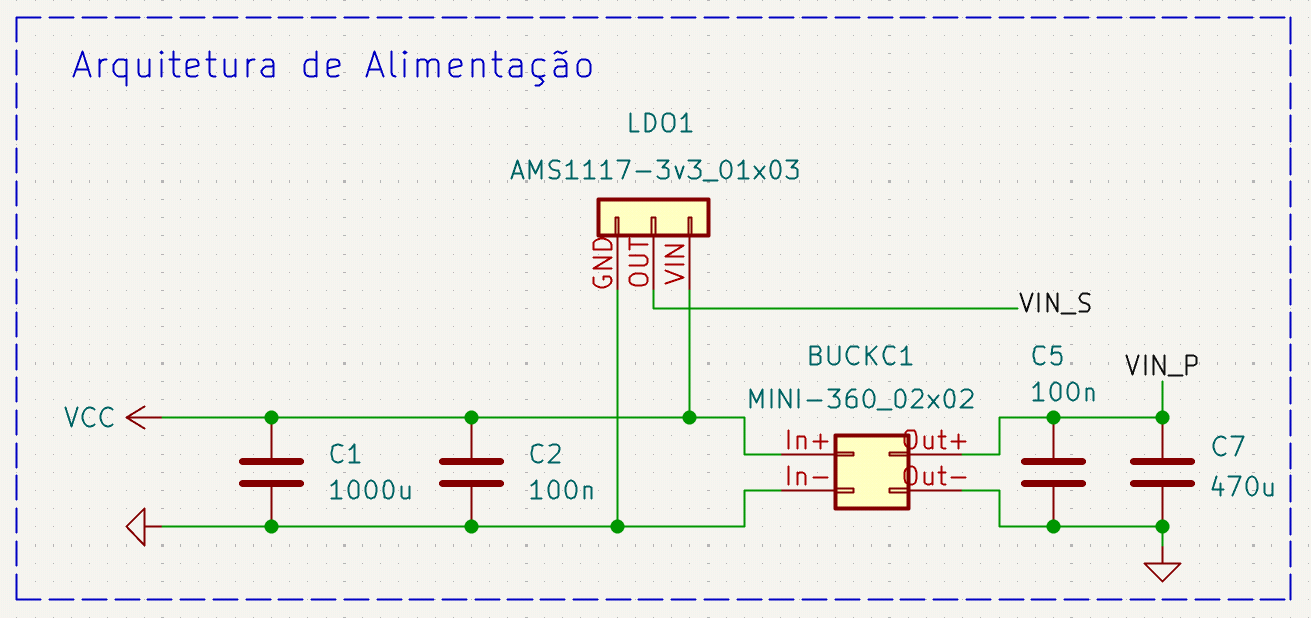
\includegraphics[width=0.9\textwidth]{images/power_scheme.png}
    \caption{Esquemático da Arquitetura de Alimentação} \label{fig:power_scheme}
\end{figure}

O desenho da arquitetura de alimentação marca o fim do processo de dimensionamento e escolha dos componentes eletrônicos. O esquemático apresentado é organizado de forma que facilite a leitura das conexões, mas não representa a disposição física dos componentes, nem o caminho exato das trilhas. Estas são funções do desenho da placa de circuito impresso (PCB), que procede o esquemático.

\section{Placa de Circuito Impresso}
Um dos maiores desafios no processo de fabricação de um sistema embarcado é a montagem do hardware. Existem algumas abordagens para esta etapa, podendo ser feita com placas de prototipagem (\textit{protoboards}), com placas cobreadas caseiras --como as placas de fenolite ou fibra de vidro laminadas com cobre--, ou ainda através da fabricação sob demanda em empresas especializadas em PCB.

Visto que o sistema irá ser embarcado em um VANT, a montagem em \textit{protoboards} está descartada. Para este projeto, será usado uma placa de fenolite duplamente cobreada, viabilizando vias nas duas faces da placa. Esta técnica é viável para produção caseira, mas exige cuidados no processo de desenho da PCB.

Os componentes podem ser adquiridos em dois níveis, conhecidos como \textit{Surface Mount Technology} (SMD) e \textit{Through Hole Technology} (THT). Placas feitas com SMD são mais compactas e com acabamento mais profissional, porém exigem a busca por distribuidores especializados que costumam vender apenas em grande quantidade. Além disso, a fabricação e manipulação de componentes SMT exigem ferramentas de precisão e prática especializada, que dificultaria e atrasaria o desenvolvimento do projeto.

Os componentes THT ocupam mais espaço e vêm prontos pra uso. Estes são mais fáceis de ter acesso e mais baratos em pequena quantidade. Além disso, a fabricação é facilitada pelos pinos que aumentam a área de contato para aplicação de estanho no processo de soldagem. Dessa forma, os componentes utilizados para este trabalho serão todos THT, valorizando a facilidade de montagem e manutenção do sistema. 

\subsection{Posicionamento dos Componentes}
Como primeiro passo para o desenho da PCB, o posicionamento dos componentes foi realizado. Para faciltar o caminho das trilhas, cada subsistema foi alocado em um espaço da placa com o cuidado de manter os limites dentro da margem do requisito RNF.03. A disposição está representada na Imagem \ref{fig:pcb_componentes}

\begin{figure}[ht]
    \centering
    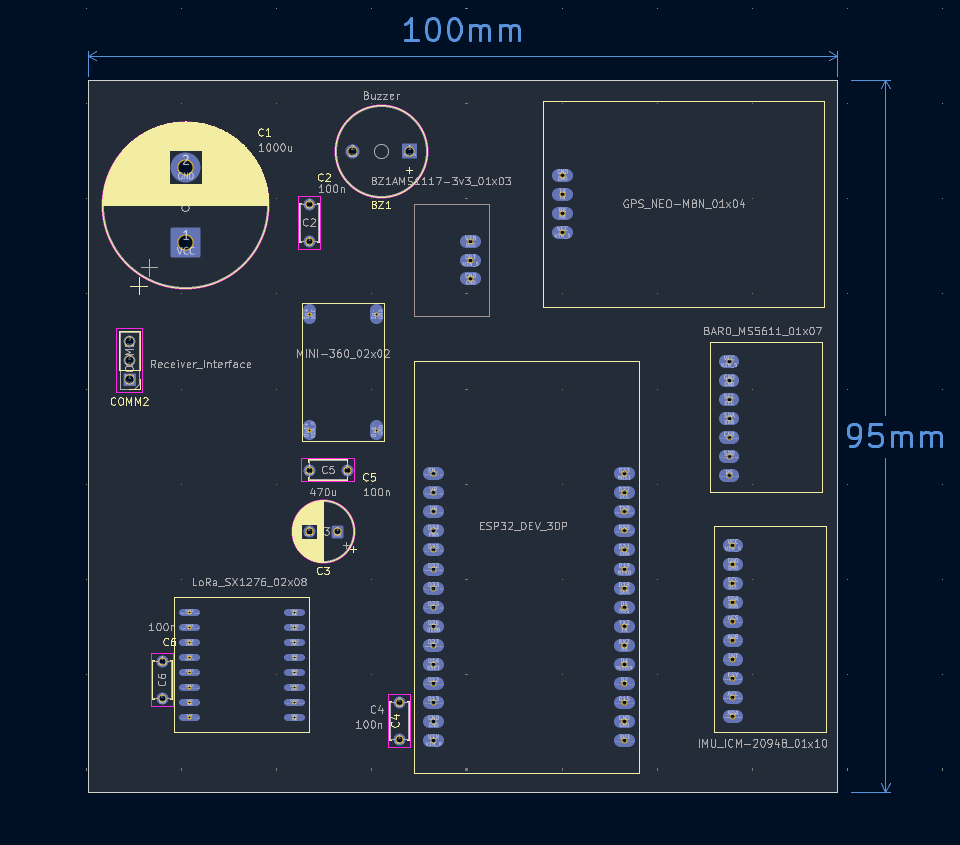
\includegraphics[width=0.8\textwidth]{images/pcb_componentes.png}
    \caption{Posicionamento dos Componentes na PCB} \label{fig:pcb_componentes}
\end{figure}

Com isso, o sistema de alimentação se concentrou ao lado esquerdo superior da face de cima da placa, com os capacitores de $100 nf$ posicionados próximo à entrada de cada componente. A entrada do PWM foi posicionada na extremidade para que o fio de acesso ao receptor comece para fora da placa. Já o SX1276 foi rotacionado de forma que sua antena fique na extremidade para facilitar a sua exposição no compartimento da aeronave.

Os sensores, ficaram ao lado contrário do sistema de alimentação para afastá-los das vias ruidosas de entrada.Em específico, o GPS foi alocado na extremidade superior direita para facilitar a integração da antena externa. Por fim, para garantir trilhas mais covenientes, o microcontrolador foi posicionado ao centro com o lado da entrada USB-C apontada para fora.

\subsection{Dimensionamento das Trilhas}
Antes de começar o desenho das trilha é importante determinar regras para garantir segurança no processo de manufatura, visto que será um processo manual. Dessa forma, determinou-se um padrão de $1 mm$ para todas as trilhas de informação e $1.8 mm$ para trilhas de alimentação. Além disso, para evitar contato entre trilhas determinou-se uma distância mínima de $0.6 mm$ entre qualquer trilha ou \textit{pad}. A partir destas regras, contruío-se as trilhas conforme Imagem \ref{fig:trilhas_pcb}, onde as trilhas vermelhas estão na face superior, e as trilhas azuis na face inferior.

\begin{figure}[ht]
    \centering
    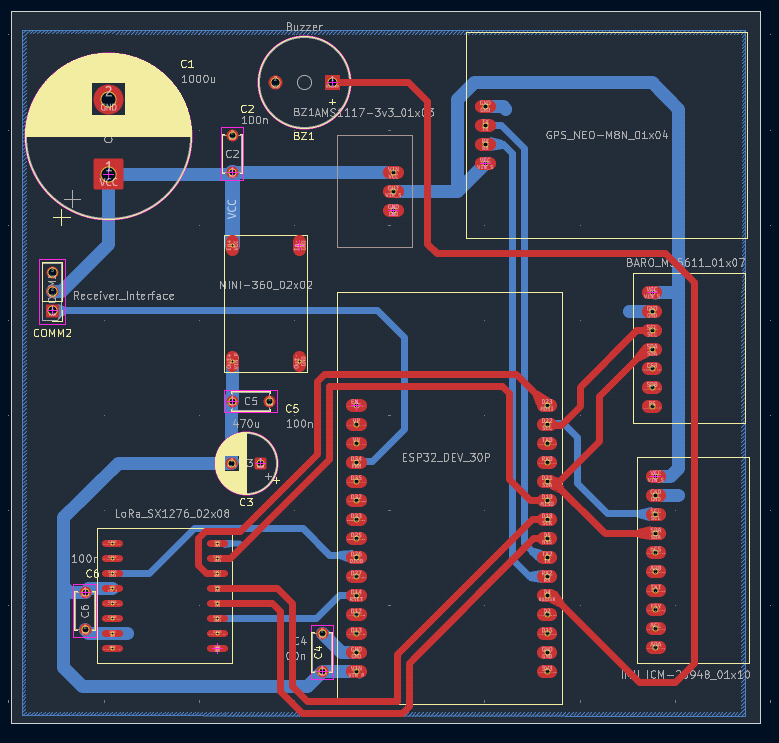
\includegraphics[width=0.8\textwidth]{images/trilhas_pcb.png}
    \caption{Disposição das Trilhas na PCB} \label{fig:trilhas_pcb}
\end{figure}

A maior parte das trilhas de informação foram posicionadas na face superior para que a face inferior fosse dedicada à zona preenchida e trilhas de alimentação. Além disso, aplicou-se o eforço de evitar trilhas com vias entre faces, ou seja, trilhas que usem as duas faces no mesmo percurso, diminuindo a complexidade construtiva da placa.

\subsection{Zona Preenchida (GND)}
Um prática comum em PCBs é a adição de uma zona preenchida para o GND. Esta estratégia cria um caminho de menor impedância para que a corrente retorne dos componentes, ajuda a proteger os sinais sensíveis de interferências eletromagnéticas, minimiza quedas de tensão, auxilia na distribuição de energia estável para todo o circuito, e ainda, reduz a quantidade de produto corrosivo no processo de corrosão da placa \cite{zona_preenchida}. Por isso, conforme Imagem \ref{fig:zona_gnd}, criou-se uma zona preenchida para o GND na face inferior da placa.

\begin{figure}[ht]
    \centering
    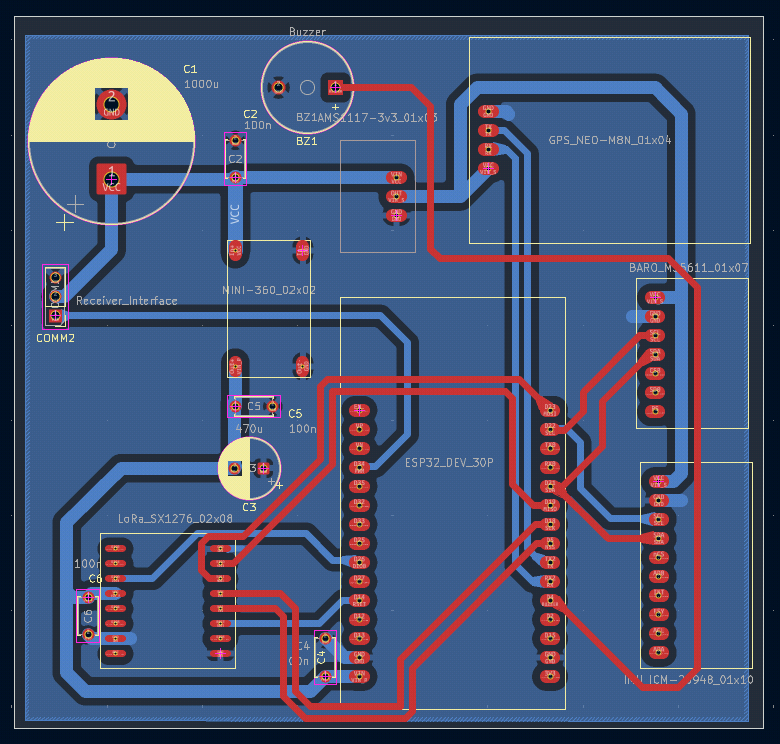
\includegraphics[width=0.8\textwidth]{images/zona_gnd.png}
    \caption{PCB com GND em Zona Preenchida} \label{fig:zona_gnd}
\end{figure}

Com isso, o desenho da PCB foi finalizado e enviado para impressão UV na placa de fenolite cobreada. Como forma de validação, conforme Imagem \ref{fig:pcb_a4} o circuito foi impresso em uma folha A4 para que os módulos pudessem ser fisicamente posicionados, validando a coerência do desenho com os componentes reais.

\begin{figure}[ht]
    \centering
    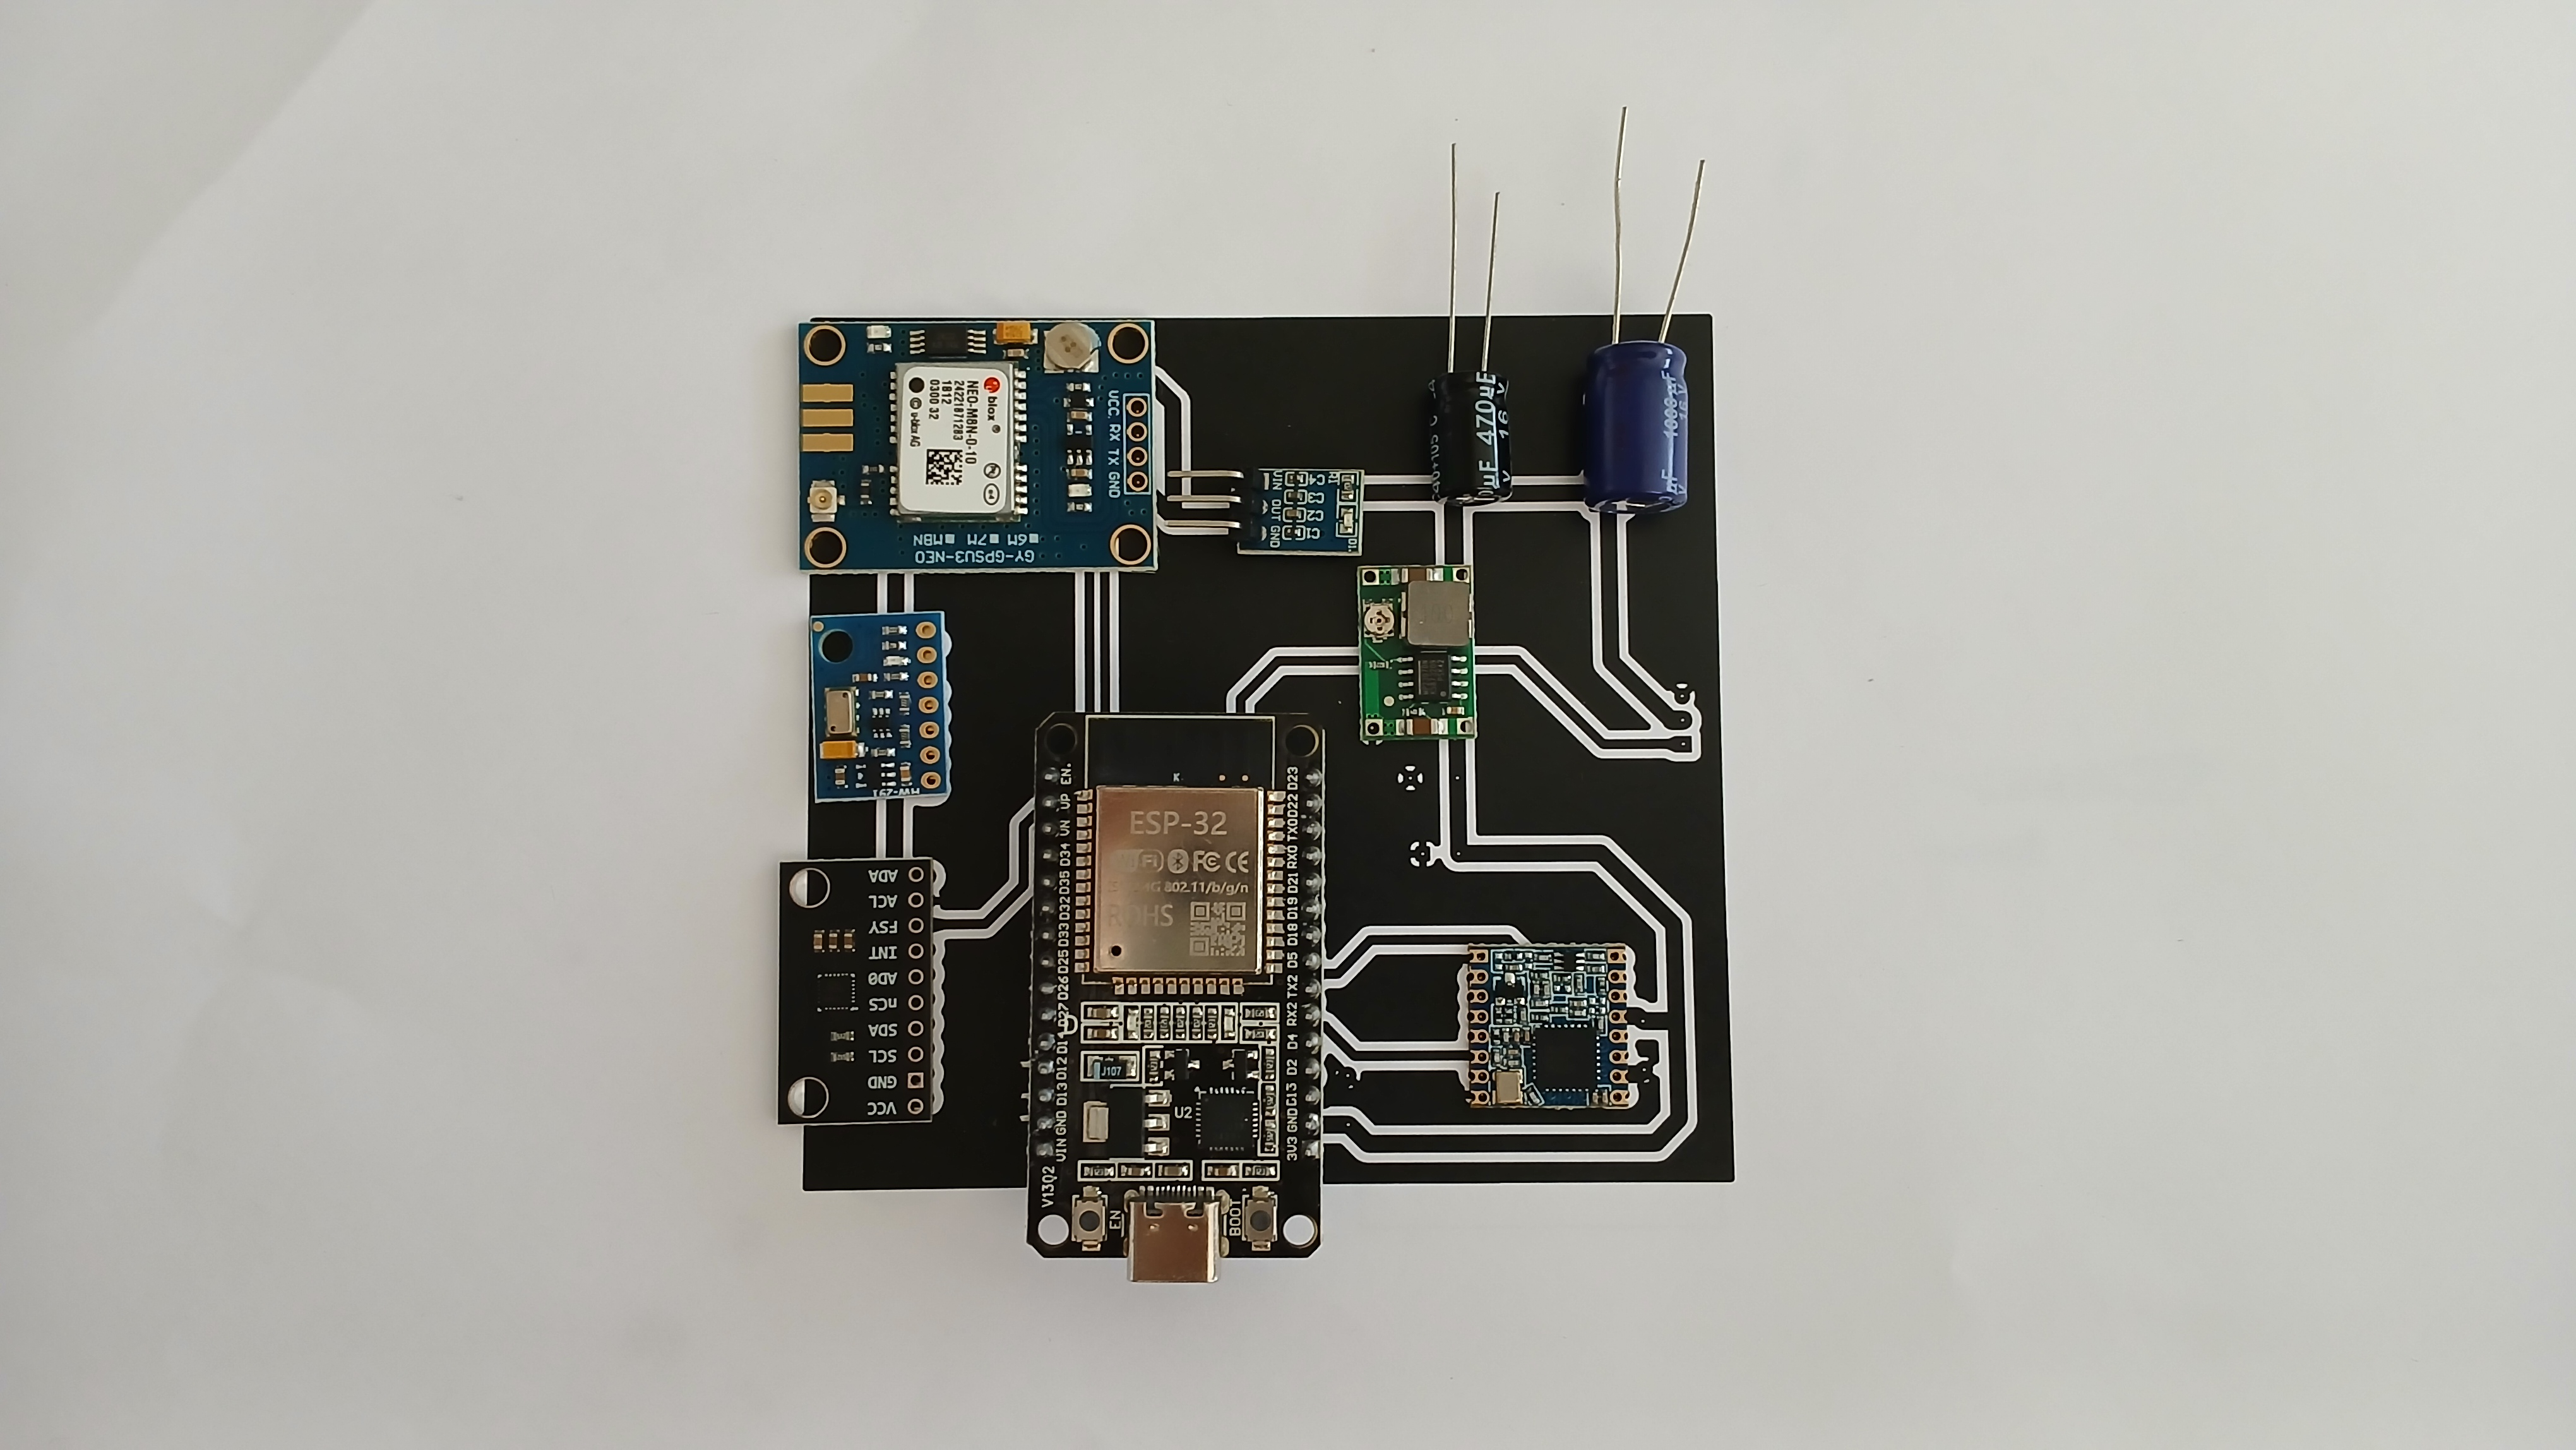
\includegraphics[width=0.9\textwidth]{images/pcb_a4.jpg}
    \caption{Validação do Posicionamento da PCB em Folha A4} \label{fig:pcb_a4}
\end{figure}

\section{\textit{Firmware}}
Para a implementação do \textit{Firmware} foram consideradas três vias de ferramentas. A primeira opção seria com programação \textit{bare-metal}, onde nenhuma camada de abstração externa é adicionada para dar total liberdade à implementação em baixíssimo nível de abstração \cite{software_embarcado}. Uma segunda alternativa é o uso de sistemas operacionais de tempo real (RTOS), que adicionam uma camada mínima para abstração de escalonamento de tarefas e gerenciamento de suas prioridades \cite{RTOS}. A última alternativa considerada foi a implementação através do framework do Arduino, que conta com suporte para ESP32 e junta diversas contribuições da comunidade, facilidade que vem em troca de performance e limitações arquiteturais. As vantagens e desvantagens de cada opção estão listadas na tabela \ref{tab:firmware_framework}.

TABELA

Além disso, o ESP-IDF é um RTOS consolidado na comunidade de desenvolvedores para ESP32, o que garante um ótimo material e robustez na ferramenta. A facilidade de implementação no Arduino Framework não compensa as limitações estabelecidas, o que atua como principal critério para eliminação desta possibilidade. Quanto ao \textit{bare-metal} há vantagens de performance, mas que não são tão promissoras em relação ao ESP-IDF, que também atua em baixo nível de abstração. 

Para um microcontrolador com dois núcleos há evidentes vantagens em usar das camadas de abstração para gerenciamento de tarefas de um sistema RTOS. Essa abordagem abre caminhos para um detalhado gerenciamento de acesso aos núcleos do ESP32, que servirá como principal estratégia para conciliar as diferentes taxas de frequência dos sensores e comunicadores.

\subsection{Arquitetura}
Visando organizar o sistema de forma a simplificar o processo de adição e/ou modificações de sensores, buscou-se arquiteturas que valorizem inversão de dependência, isolando a regra de negócio das especificidades de cada componente. Para isso, uma opção com grande potencial é a arquitetura hexagonal --também conhecida como arquitetura \textit{ports and adapters}, que se divide em três partes principais: \textit{domain}, \textit{ports} e \textit{adapters} \cite{arquitetura_hexagonal}.

Nesta arquitetura, o \textit{domain} será uma camada de lógica de negócios, agnóstica a técnologias. Ou seja, será uma camada para implementação em C++ puro que não conhecerá quais serão os componentes de hardware. Para que o \textit{domain} se comunique com as tecnologias externas, as \textit{ports} servirão de camada de abstração, fornecendo interfaces com os contratos que o \textit{domain} sabe usar. Por fim, os \textit{adapters} serão os componentes externos à camada central e implementarão as interfaces das \textit{ports} seguindo as especificações de cada hardware, sejam estes sensores, comunicadores ou o próprio microcontrolador. A distribuição das camadas está descrita de forma visual no diagrama da Imagem \ref{fig:diagrama_hexagonal}.

Com isso, a arquitetura servirá não apenas de guia, mas também como rigor de projeto que deve ser respeitado para manter a manutenabilidade e escalabilidade do sistema.

\subsection{Camada \textit{Domain}}
Lógica de negócios

\subsection{Comunicação com piloto}
Sistema PWM, acesso do rádio controle e buzzer

\subsection{Leitura dos sensores}
Camada de adapter e ports para os sensores

\subsection{Tratamento de dados na ponta}
Filtros, edge computing, redução de carga na rede

\subsection{Transmissão e arquivamento das leituras}
Transmissão via LoRa e escrita no cartão SD

\subsection{Detalhes técnicos}
Detalhes de implementação que merecem destaque


\section{Protótipo}
Processo de fabricação, teste e estimativa de consumo elétrico

